\chapter{Les Architectures proposées pour la Segmentation d’images Biomédicales}
\lhead{\textit{Chapitre \thechapter}}
\rhead{\textit{Les architectures proposées}}


\section{Introduction}
Lorem ipsum dolor sit amet, consectetur adipiscing elit. Curabitur a ullamcorper purus, sit amet cursus turpis. Nullam ipsum nibh, imperdiet vitae hendrerit et, porta sit amet lorem. In eu sem viverra, condimentum enim ac, congue dui. Quisque quis urna et quam vehicula tristique a a dui. Vestibulum euismod malesuada maximus. Vivamus vel lacinia nisi. Suspendisse ac fermentum ante, vel condimentum odio. Praesent ut nibh tempor, condimentum eros sit amet, scelerisque sapien. Nam ut nisl sit amet risus viverra fringilla quis a sapien. Curabitur id quam nisl. Sed volutpat varius neque eget tempor. Proin eget ultrices magna, ullamcorper ultricies leo. Suspendisse vitae ex sit amet dolor venenatis imperdiet non sit amet turpis. Vestibulum ante ipsum primis in faucibus orci luctus et ultrices posuere cubilia curae; Nulla quis suscipit ipsum. In rhoncus urna a quam eleifend, vitae euismod tellus varius.
\newpage
\section{Description de la solution proposée}
Lorem ipsum dolor sit amet, consectetur adipiscing elit. Curabitur a ullamcorper purus, sit amet cursus turpis. Nullam ipsum nibh, imperdiet vitae hendrerit et, porta sit amet lorem. In eu sem viverra, condimentum enim ac, congue dui. Quisque quis urna et quam vehicula tristique a a dui. Vestibulum euismod malesuada maximus. Vivamus vel lacinia nisi. Suspendisse ac fermentum ante, vel condimentum odio. Praesent ut nibh tempor, condimentum eros sit amet, scelerisque sapien. Nam ut nisl sit amet risus viverra fringilla quis a sapien. Curabitur id quam nisl. Sed volutpat varius neque eget tempor. Proin eget ultrices magna, ullamcorper ultricies leo. Suspendisse vitae ex sit amet dolor venenatis imperdiet non sit amet turpis. Vestibulum ante ipsum primis in faucibus orci luctus et ultrices posuere cubilia curae; Nulla quis suscipit ipsum. In rhoncus urna a quam eleifend, vitae euismod tellus varius.
\vspace{10pt}

\subsection{Architecture U-Net: }
U-Net développée par Zhengxin Zhang et al.
\footnote{U-Net: Convolutional Networks for Biomedical Image Segmentation\newline https://arxiv.org/pdf/1505.04597.pdf} en 2015, était un CNN unique développé pour la segmentation d'images biomédicales,est maintenant devenu un réseau d'encodeur-décodeur très populaire pour la segmentation sémantique il a une architecture UP-Down unique qui a un chemin Contractuel et un chemin Expansif.
\vspace{10pt}
\begin{figure*}[htp]
    \centering
    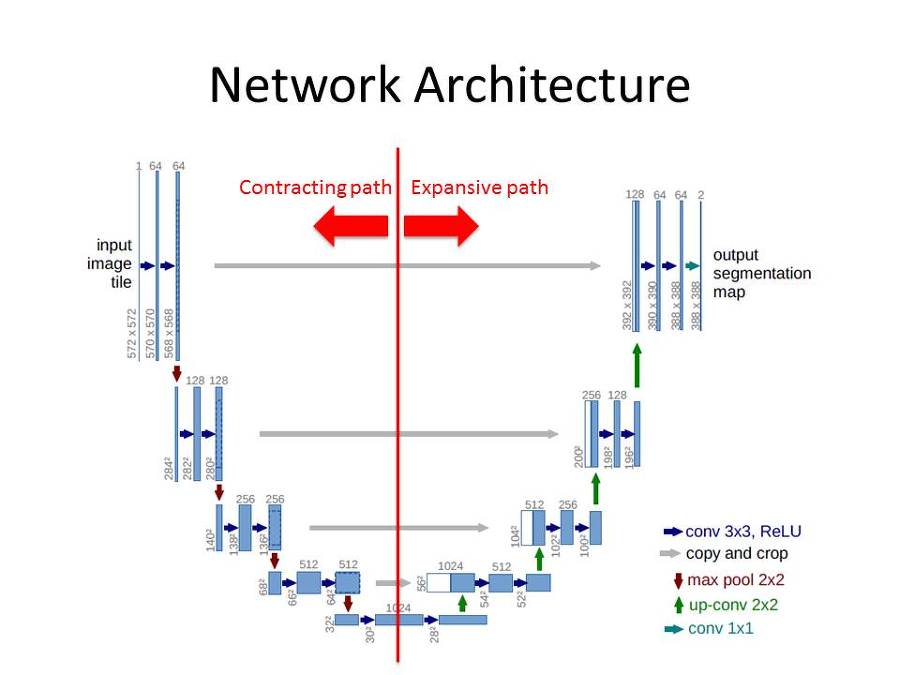
\includegraphics[width=10cm]{Chapiters/Chapiter_03/Pictures/unet.jpg}
    \caption{Architecture U-Net}
    \label{unet}
\end{figure*}
\newpage
\section{Conclusion}
Lorem ipsum dolor sit amet, consectetur adipiscing elit. Curabitur a ullamcorper purus, sit amet cursus turpis. Nullam ipsum nibh, imperdiet vitae hendrerit et, porta sit amet lorem. In eu sem viverra, condimentum enim ac, congue dui. Quisque quis urna et quam vehicula tristique a a dui. Vestibulum euismod malesuada maximus. Vivamus vel lacinia nisi. Suspendisse ac fermentum ante, vel condimentum odio. Praesent ut nibh tempor, condimentum eros sit amet, scelerisque sapien. Nam ut nisl sit amet risus viverra fringilla quis a sapien. Curabitur id quam nisl. Sed volutpat varius neque eget tempor. Proin eget ultrices magna, ullamcorper ultricies leo. Suspendisse vitae ex sit amet dolor venenatis imperdiet non sit amet turpis. Vestibulum ante ipsum primis in faucibus orci luctus et ultrices posuere cubilia curae; Nulla quis suscipit ipsum. In rhoncus urna a quam eleifend, vitae euismod tellus varius. 